%%%%%%%%%%%%%%%%%%%%%%%%%%%%%%%%%%%%%%%%%
% The Legrand Orange Book
% LaTeX Template
% Version 2.2 (30/3/17)
%
% This template has been downloaded from:
% http://www.LaTeXTemplates.com
%
% Original author:
% Mathias Legrand (legrand.mathias@gmail.com) with modifications by:
% Vel (vel@latextemplates.com)
%
% License:
% CC BY-NC-SA 3.0 (http://creativecommons.org/licenses/by-nc-sa/3.0/)
%
% Compiling this template:
% This template uses biber for its bibliography and makeindex for its index.
% When you first open the template, compile it from the command line with the
% commands below to make sure your LaTeX distribution is configured correctly:
%
% 1) pdflatex main
% 2) makeindex main.idx -s StyleInd.ist
% 3) biber main
% 4) pdflatex main x 2
%
% After this, when you wish to update the bibliography/index use the appropriate
% command above and make sure to compile with pdflatex several times
% afterwards to propagate your changes to the document.
%
% This template also uses a number of packages which may need to be
% updated to the newest versions for the template to compile. It is strongly
% recommended you update your LaTeX distribution if you have any
% compilation errors.
%
% Important note:
% Chapter heading images should have a 2:1 width:height ratio,
% e.g. 920px width and 460px height.
%
%%%%%%%%%%%%%%%%%%%%%%%%%%%%%%%%%%%%%%%%%

%----------------------------------------------------------------------------------------
%	PACKAGES AND OTHER DOCUMENT CONFIGURATIONS
%----------------------------------------------------------------------------------------

\documentclass[11pt]{book} % Default font size and left-justified equations

%----------------------------------------------------------------------------------------

%%%%%%%%%%%%%%%%%%%%%%%%%%%%%%%%%%%%%%%%%
% The Legrand Orange Book
% Structural Definitions File
% Version 2.0 (9/2/15)
%
% Original author:
% Mathias Legrand (legrand.mathias@gmail.com) with modifications by:
% Vel (vel@latextemplates.com)
% 
% This file has been downloaded from:
% http://www.LaTeXTemplates.com
%
% License:
% CC BY-NC-SA 3.0 (http://creativecommons.org/licenses/by-nc-sa/3.0/)
%
%%%%%%%%%%%%%%%%%%%%%%%%%%%%%%%%%%%%%%%%%

%----------------------------------------------------------------------------------------
%	VARIOUS REQUIRED PACKAGES AND CONFIGURATIONS
%----------------------------------------------------------------------------------------

\usepackage[top=3cm,bottom=3cm,left=3cm,right=3cm,headsep=10pt,a4paper]{geometry} % Page margins

\usepackage{graphicx} % Required for including pictures
\graphicspath{{Pictures/}} % Specifies the directory where pictures are stored

\usepackage{lipsum} % Inserts dummy text

\usepackage{tikz} % Required for drawing custom shapes

\usepackage[english]{babel} % English language/hyphenation

\usepackage{enumitem} % Customize lists
\setlist{nolistsep} % Reduce spacing between bullet points and numbered lists

\usepackage{booktabs} % Required for nicer horizontal rules in tables

\usepackage{xcolor} % Required for specifying colors by name
\definecolor{steelblue}{RGB}{70,70,230} % Define the orange color used for highlighting throughout the book


%----------------------------------------------------------------------------------------
%	FONTS
%----------------------------------------------------------------------------------------

\usepackage{avant} % Use the Avantgarde font for headings
%\usepackage{times} % Use the Times font for headings
\usepackage{mathptmx} % Use the Adobe Times Roman as the default text font together with math symbols from the Sym­bol, Chancery and Com­puter Modern fonts

\usepackage{microtype} % Slightly tweak font spacing for aesthetics
\usepackage[utf8]{inputenc} % Required for including letters with accents
\usepackage[T1]{fontenc} % Use 8-bit encoding that has 256 glyphs

%----------------------------------------------------------------------------------------
%	BIBLIOGRAPHY AND INDEX
%----------------------------------------------------------------------------------------

\usepackage[style=alphabetic,citestyle=numeric,sorting=nyt,sortcites=true,autopunct=true,babel=hyphen,hyperref=true,abbreviate=false,backref=true,backend=biber]{biblatex}
\addbibresource{bibliography.bib} % BibTeX bibliography file
\defbibheading{bibempty}{}

\usepackage{calc} % For simpler calculation - used for spacing the index letter headings correctly
\usepackage{makeidx} % Required to make an index
\makeindex % Tells LaTeX to create the files required for indexing

%----------------------------------------------------------------------------------------
%	MAIN TABLE OF CONTENTS
%----------------------------------------------------------------------------------------

\usepackage{titletoc} % Required for manipulating the table of contents

\contentsmargin{0cm} % Removes the default margin

% Part text styling
\titlecontents{part}[0cm]
{\addvspace{20pt}\centering\large\bfseries}
{}
{}
{}

% Chapter text styling
\titlecontents{chapter}[1.25cm] % Indentation
{\addvspace{12pt}\large\sffamily\bfseries} % Spacing and font options for chapters
{\color{steelblue!60}\contentslabel[\Large\thecontentslabel]{1.25cm}\color{steelblue}} % Chapter number
{\color{steelblue}}  
{\color{steelblue!60}\normalsize\;\titlerule*[.5pc]{.}\;\thecontentspage} % Page number

% Section text styling
\titlecontents{section}[1.25cm] % Indentation
{\addvspace{3pt}\sffamily\bfseries} % Spacing and font options for sections
{\contentslabel[\thecontentslabel]{1.25cm}} % Section number
{}
{\hfill\color{black}\thecontentspage} % Page number
[]

% Subsection text styling
\titlecontents{subsection}[1.25cm] % Indentation
{\addvspace{1pt}\sffamily\small} % Spacing and font options for subsections
{\contentslabel[\thecontentslabel]{1.25cm}} % Subsection number
{}
{\ \titlerule*[.5pc]{.}\;\thecontentspage} % Page number
[]

% List of figures
\titlecontents{figure}[0em]
{\addvspace{-5pt}\sffamily}
{\thecontentslabel\hspace*{1em}}
{}
{\ \titlerule*[.5pc]{.}\;\thecontentspage}
[]

% List of tables
\titlecontents{table}[0em]
{\addvspace{-5pt}\sffamily}
{\thecontentslabel\hspace*{1em}}
{}
{\ \titlerule*[.5pc]{.}\;\thecontentspage}
[]

%----------------------------------------------------------------------------------------
%	MINI TABLE OF CONTENTS IN PART HEADS
%----------------------------------------------------------------------------------------

% Chapter text styling
\titlecontents{lchapter}[0em] % Indenting
{\addvspace{15pt}\large\sffamily\bfseries} % Spacing and font options for chapters
{\color{steelblue}\contentslabel[\Large\thecontentslabel]{1.25cm}\color{steelblue}} % Chapter number
{}  
{\color{steelblue}\normalsize\sffamily\bfseries\;\titlerule*[.5pc]{.}\;\thecontentspage} % Page number

% Section text styling
\titlecontents{lsection}[0em] % Indenting
{\sffamily\small} % Spacing and font options for sections
{\contentslabel[\thecontentslabel]{1.25cm}} % Section number
{}
{}

% Subsection text styling
\titlecontents{lsubsection}[.5em] % Indentation
{\normalfont\footnotesize\sffamily} % Font settings
{}
{}
{}

%----------------------------------------------------------------------------------------
%	PAGE HEADERS
%----------------------------------------------------------------------------------------

\usepackage{fancyhdr} % Required for header and footer configuration

\pagestyle{fancy}
\renewcommand{\chaptermark}[1]{\markboth{\sffamily\normalsize\bfseries\chaptername\ \thechapter.\ #1}{}} % Chapter text font settings
\renewcommand{\sectionmark}[1]{\markright{\sffamily\normalsize\thesection\hspace{5pt}#1}{}} % Section text font settings
\fancyhf{} \fancyhead[LE,RO]{\sffamily\normalsize\thepage} % Font setting for the page number in the header
\fancyhead[LO]{\rightmark} % Print the nearest section name on the left side of odd pages
\fancyhead[RE]{\leftmark} % Print the current chapter name on the right side of even pages
\renewcommand{\headrulewidth}{0.5pt} % Width of the rule under the header
\addtolength{\headheight}{2.5pt} % Increase the spacing around the header slightly
\renewcommand{\footrulewidth}{0pt} % Removes the rule in the footer
\fancypagestyle{plain}{\fancyhead{}\renewcommand{\headrulewidth}{0pt}} % Style for when a plain pagestyle is specified

% Removes the header from odd empty pages at the end of chapters
\makeatletter
\renewcommand{\cleardoublepage}{
\clearpage\ifodd\c@page\else
\hbox{}
\vspace*{\fill}
\thispagestyle{empty}
\newpage
\fi}

%----------------------------------------------------------------------------------------
%	THEOREM STYLES
%----------------------------------------------------------------------------------------

\usepackage{amsmath,amsfonts,amssymb,amsthm} % For math equations, theorems, symbols, etc

\newcommand{\intoo}[2]{\mathopen{]}#1\,;#2\mathclose{[}}
\newcommand{\ud}{\mathop{\mathrm{{}d}}\mathopen{}}
\newcommand{\intff}[2]{\mathopen{[}#1\,;#2\mathclose{]}}
\newtheorem{notation}{Notation}[chapter]

% Boxed/framed environments
\newtheoremstyle{steelbluenumbox}% % Theorem style name
{0pt}% Space above
{0pt}% Space below
{\normalfont}% % Body font
{}% Indent amount
{\small\bf\sffamily\color{steelblue}}% % Theorem head font
{\;}% Punctuation after theorem head
{0.25em}% Space after theorem head
{\small\sffamily\color{steelblue}\thmname{#1}\nobreakspace\thmnumber{\@ifnotempty{#1}{}\@upn{#2}}% Theorem text (e.g. Theorem 2.1)
\thmnote{\nobreakspace\the\thm@notefont\sffamily\bfseries\color{black}---\nobreakspace#3.}} % Optional theorem note
\renewcommand{\qedsymbol}{$\blacksquare$}% Optional qed square

\newtheoremstyle{blacknumex}% Theorem style name
{5pt}% Space above
{5pt}% Space below
{\normalfont}% Body font
{} % Indent amount
{\small\bf\sffamily}% Theorem head font
{\;}% Punctuation after theorem head
{0.25em}% Space after theorem head
{\small\sffamily{\tiny\ensuremath{\blacksquare}}\nobreakspace\thmname{#1}\nobreakspace\thmnumber{\@ifnotempty{#1}{}\@upn{#2}}% Theorem text (e.g. Theorem 2.1)
\thmnote{\nobreakspace\the\thm@notefont\sffamily\bfseries---\nobreakspace#3.}}% Optional theorem note

\newtheoremstyle{blacknumbox} % Theorem style name
{0pt}% Space above
{0pt}% Space below
{\normalfont}% Body font
{}% Indent amount
{\small\bf\sffamily}% Theorem head font
{\;}% Punctuation after theorem head
{0.25em}% Space after theorem head
{\small\sffamily\thmname{#1}\nobreakspace\thmnumber{\@ifnotempty{#1}{}\@upn{#2}}% Theorem text (e.g. Theorem 2.1)
\thmnote{\nobreakspace\the\thm@notefont\sffamily\bfseries---\nobreakspace#3.}}% Optional theorem note

% Non-boxed/non-framed environments
\newtheoremstyle{steelbluenum}% % Theorem style name
{5pt}% Space above
{5pt}% Space below
{\normalfont}% % Body font
{}% Indent amount
{\small\bf\sffamily\color{steelblue}}% % Theorem head font
{\;}% Punctuation after theorem head
{0.25em}% Space after theorem head
{\small\sffamily\color{steelblue}\thmname{#1}\nobreakspace\thmnumber{\@ifnotempty{#1}{}\@upn{#2}}% Theorem text (e.g. Theorem 2.1)
\thmnote{\nobreakspace\the\thm@notefont\sffamily\bfseries\color{black}---\nobreakspace#3.}} % Optional theorem note
\renewcommand{\qedsymbol}{$\blacksquare$}% Optional qed square
\makeatother

% Defines the theorem text style for each type of theorem to one of the three styles above
\newcounter{dummy} 
\numberwithin{dummy}{section}
\theoremstyle{steelbluenumbox}
\newtheorem{theoremeT}[dummy]{Theorem}
\newtheorem{problem}{Problem}[chapter]
\newtheorem{exerciseT}{Exercise}[chapter]
\theoremstyle{blacknumex}
\newtheorem{exampleT}{Example}[chapter]
\theoremstyle{blacknumbox}
\newtheorem{vocabulary}{Vocabulary}[chapter]
\newtheorem{definitionT}{Definition}[section]
\newtheorem{corollaryT}[dummy]{Corollary}
\theoremstyle{steelbluenum}
\newtheorem{proposition}[dummy]{Proposition}

%----------------------------------------------------------------------------------------
%	DEFINITION OF COLORED BOXES
%----------------------------------------------------------------------------------------

\RequirePackage[framemethod=default]{mdframed} % Required for creating the theorem, definition, exercise and corollary boxes

% Theorem box
\newmdenv[skipabove=7pt,
skipbelow=7pt,
backgroundcolor=black!5,
linecolor=steelblue,
innerleftmargin=5pt,
innerrightmargin=5pt,
innertopmargin=5pt,
leftmargin=0cm,
rightmargin=0cm,
innerbottommargin=5pt]{tBox}

% Exercise box	  
\newmdenv[skipabove=7pt,
skipbelow=7pt,
rightline=false,
leftline=true,
topline=false,
bottomline=false,
backgroundcolor=steelblue!10,
linecolor=steelblue,
innerleftmargin=5pt,
innerrightmargin=5pt,
innertopmargin=5pt,
innerbottommargin=5pt,
leftmargin=0cm,
rightmargin=0cm,
linewidth=4pt]{eBox}	

% Definition box
\newmdenv[skipabove=7pt,
skipbelow=7pt,
rightline=false,
leftline=true,
topline=false,
bottomline=false,
linecolor=steelblue,
innerleftmargin=5pt,
innerrightmargin=5pt,
innertopmargin=0pt,
leftmargin=0cm,
rightmargin=0cm,
linewidth=4pt,
innerbottommargin=0pt]{dBox}	

% Corollary box
\newmdenv[skipabove=7pt,
skipbelow=7pt,
rightline=false,
leftline=true,
topline=false,
bottomline=false,
linecolor=gray,
backgroundcolor=black!5,
innerleftmargin=5pt,
innerrightmargin=5pt,
innertopmargin=5pt,
leftmargin=0cm,
rightmargin=0cm,
linewidth=4pt,
innerbottommargin=5pt]{cBox}

% Creates an environment for each type of theorem and assigns it a theorem text style from the "Theorem Styles" section above and a colored box from above
\newenvironment{theorem}{\begin{tBox}\begin{theoremeT}}{\end{theoremeT}\end{tBox}}
\newenvironment{exercise}{\begin{eBox}\begin{exerciseT}}{\hfill{\color{steelblue}\tiny\ensuremath{\blacksquare}}\end{exerciseT}\end{eBox}}				  
\newenvironment{definition}{\begin{dBox}\begin{definitionT}}{\end{definitionT}\end{dBox}}	
\newenvironment{example}{\begin{exampleT}}{\hfill{\tiny\ensuremath{\blacksquare}}\end{exampleT}}		
\newenvironment{corollary}{\begin{cBox}\begin{corollaryT}}{\end{corollaryT}\end{cBox}}	

%----------------------------------------------------------------------------------------
%	REMARK ENVIRONMENT
%----------------------------------------------------------------------------------------

\newenvironment{remark}{\par\vspace{10pt}\small % Vertical white space above the remark and smaller font size
\begin{list}{}{
\leftmargin=35pt % Indentation on the left
\rightmargin=25pt}\item\ignorespaces % Indentation on the right
\makebox[-2.5pt]{\begin{tikzpicture}[overlay]
\node[draw=steelblue!60,line width=1pt,circle,fill=steelblue!25,font=\sffamily\bfseries,inner sep=2pt,outer sep=0pt] at (-15pt,0pt){\textcolor{steelblue}{R}};\end{tikzpicture}} % Orange R in a circle
\advance\baselineskip -1pt}{\end{list}\vskip5pt} % Tighter line spacing and white space after remark

%----------------------------------------------------------------------------------------
%	SECTION NUMBERING IN THE MARGIN
%----------------------------------------------------------------------------------------

\makeatletter
\renewcommand{\@seccntformat}[1]{\llap{\textcolor{steelblue}{\csname the#1\endcsname}\hspace{1em}}}                    
\renewcommand{\section}{\@startsection{section}{1}{\z@}
{-4ex \@plus -1ex \@minus -.4ex}
{1ex \@plus.2ex }
{\normalfont\large\sffamily\bfseries}}
\renewcommand{\subsection}{\@startsection {subsection}{2}{\z@}
{-3ex \@plus -0.1ex \@minus -.4ex}
{0.5ex \@plus.2ex }
{\normalfont\sffamily\bfseries}}
\renewcommand{\subsubsection}{\@startsection {subsubsection}{3}{\z@}
{-2ex \@plus -0.1ex \@minus -.2ex}
{.2ex \@plus.2ex }
{\normalfont\small\sffamily\bfseries}}                        
\renewcommand\paragraph{\@startsection{paragraph}{4}{\z@}
{-2ex \@plus-.2ex \@minus .2ex}
{.1ex}
{\normalfont\small\sffamily\bfseries}}

%----------------------------------------------------------------------------------------
%	PART HEADINGS
%----------------------------------------------------------------------------------------

% numbered part in the table of contents
\newcommand{\@mypartnumtocformat}[2]{%
\setlength\fboxsep{0pt}%
\noindent\colorbox{steelblue!20}{\strut\parbox[c][.7cm]{\ecart}{\color{steelblue!70}\Large\sffamily\bfseries\centering#1}}\hskip\esp\colorbox{steelblue!40}{\strut\parbox[c][.7cm]{\linewidth-\ecart-\esp}{\Large\sffamily\centering#2}}}%
%%%%%%%%%%%%%%%%%%%%%%%%%%%%%%%%%%
% unnumbered part in the table of contents
\newcommand{\@myparttocformat}[1]{%
\setlength\fboxsep{0pt}%
\noindent\colorbox{steelblue!40}{\strut\parbox[c][.7cm]{\linewidth}{\Large\sffamily\centering#1}}}%
%%%%%%%%%%%%%%%%%%%%%%%%%%%%%%%%%%
\newlength\esp
\setlength\esp{4pt}
\newlength\ecart
\setlength\ecart{1.2cm-\esp}
\newcommand{\thepartimage}{}%
\newcommand{\partimage}[1]{\renewcommand{\thepartimage}{#1}}%
\def\@part[#1]#2{%
\ifnum \c@secnumdepth >-2\relax%
\refstepcounter{part}%
\addcontentsline{toc}{part}{\texorpdfstring{\protect\@mypartnumtocformat{\thepart}{#1}}{\partname~\thepart\ ---\ #1}}
\else%
\addcontentsline{toc}{part}{\texorpdfstring{\protect\@myparttocformat{#1}}{#1}}%
\fi%
\startcontents%
\markboth{}{}%
{\thispagestyle{empty}%
\begin{tikzpicture}[remember picture,overlay]%
\node at (current page.north west){\begin{tikzpicture}[remember picture,overlay]%	
\fill[steelblue!20](0cm,0cm) rectangle (\paperwidth,-\paperheight);
\node[anchor=north] at (4cm,-3.25cm){\color{steelblue!40}\fontsize{220}{100}\sffamily\bfseries\thepart}; 
\node[anchor=south east] at (\paperwidth-1cm,-\paperheight+1cm){\parbox[t][][t]{8.5cm}{
\printcontents{l}{0}{\setcounter{tocdepth}{1}}%
}};
\node[anchor=north east] at (\paperwidth-1.5cm,-3.25cm){\parbox[t][][t]{15cm}{\strut\raggedleft\color{white}\fontsize{30}{30}\sffamily\bfseries#2}};
\end{tikzpicture}};
\end{tikzpicture}}%
\@endpart}
\def\@spart#1{%
\startcontents%
\phantomsection
{\thispagestyle{empty}%
\begin{tikzpicture}[remember picture,overlay]%
\node at (current page.north west){\begin{tikzpicture}[remember picture,overlay]%	
\fill[steelblue!20](0cm,0cm) rectangle (\paperwidth,-\paperheight);
\node[anchor=north east] at (\paperwidth-1.5cm,-3.25cm){\parbox[t][][t]{15cm}{\strut\raggedleft\color{white}\fontsize{30}{30}\sffamily\bfseries#1}};
\end{tikzpicture}};
\end{tikzpicture}}
\addcontentsline{toc}{part}{\texorpdfstring{%
\setlength\fboxsep{0pt}%
\noindent\protect\colorbox{steelblue!40}{\strut\protect\parbox[c][.7cm]{\linewidth}{\Large\sffamily\protect\centering #1\quad\mbox{}}}}{#1}}%
\@endpart}
\def\@endpart{\vfil\newpage
\if@twoside
\if@openright
\null
\thispagestyle{empty}%
\newpage
\fi
\fi
\if@tempswa
\twocolumn
\fi}

%----------------------------------------------------------------------------------------
%	CHAPTER HEADINGS
%----------------------------------------------------------------------------------------

% A switch to conditionally include a picture, implemented by  Christian Hupfer
\newif\ifusechapterimage
\usechapterimagetrue
\newcommand{\thechapterimage}{}%
\newcommand{\chapterimage}[1]{\ifusechapterimage\renewcommand{\thechapterimage}{#1}\fi}%
\newcommand{\autodot}{.}
\def\@makechapterhead#1{%
{\parindent \z@ \raggedright \normalfont
\ifnum \c@secnumdepth >\m@ne
\if@mainmatter
\begin{tikzpicture}[remember picture,overlay]
\node at (current page.north west)
{\begin{tikzpicture}[remember picture,overlay]
\node[anchor=north west,inner sep=0pt] at (0,0) {\ifusechapterimage\includegraphics[width=\paperwidth]{\thechapterimage}\fi};
\draw[anchor=west] (\Gm@lmargin,-9cm) node [line width=2pt,rounded corners=15pt,draw=steelblue,fill=white,fill opacity=0.5,inner sep=15pt]{\strut\makebox[22cm]{}};
\draw[anchor=west] (\Gm@lmargin+.3cm,-9cm) node {\huge\sffamily\bfseries\color{black}\thechapter\autodot~#1\strut};
\end{tikzpicture}};
\end{tikzpicture}
\else
\begin{tikzpicture}[remember picture,overlay]
\node at (current page.north west)
{\begin{tikzpicture}[remember picture,overlay]
\node[anchor=north west,inner sep=0pt] at (0,0) {\ifusechapterimage\includegraphics[width=\paperwidth]{\thechapterimage}\fi};
\draw[anchor=west] (\Gm@lmargin,-9cm) node [line width=2pt,rounded corners=15pt,draw=steelblue,fill=white,fill opacity=0.5,inner sep=15pt]{\strut\makebox[22cm]{}};
\draw[anchor=west] (\Gm@lmargin+.3cm,-9cm) node {\huge\sffamily\bfseries\color{black}#1\strut};
\end{tikzpicture}};
\end{tikzpicture}
\fi\fi\par\vspace*{270\p@}}}

%-------------------------------------------

\def\@makeschapterhead#1{%
\begin{tikzpicture}[remember picture,overlay]
\node at (current page.north west)
{\begin{tikzpicture}[remember picture,overlay]
\node[anchor=north west,inner sep=0pt] at (0,0) {\ifusechapterimage\includegraphics[width=\paperwidth]{\thechapterimage}\fi};
\draw[anchor=west] (\Gm@lmargin,-9cm) node [line width=2pt,rounded corners=15pt,draw=steelblue,fill=white,fill opacity=0.5,inner sep=15pt]{\strut\makebox[22cm]{}};
\draw[anchor=west] (\Gm@lmargin+.3cm,-9cm) node {\huge\sffamily\bfseries\color{black}#1\strut};
\end{tikzpicture}};
\end{tikzpicture}
\par\vspace*{270\p@}}
\makeatother

%----------------------------------------------------------------------------------------
%	HYPERLINKS IN THE DOCUMENTS
%----------------------------------------------------------------------------------------

\usepackage{hyperref}
\hypersetup{hidelinks,backref=true,pagebackref=true,hyperindex=true,colorlinks=false,breaklinks=true,urlcolor= steelblue,bookmarks=true,bookmarksopen=false,pdftitle={Title},pdfauthor={Author}}
\usepackage{bookmark}
\bookmarksetup{
open,
numbered,
addtohook={%
\ifnum\bookmarkget{level}=0 % chapter
\bookmarksetup{bold}%
\fi
\ifnum\bookmarkget{level}=-1 % part
\bookmarksetup{color=steelblue,bold}%
\fi
}
}
 % Insert the commands.tex file which contains the majority of the structure behind the template

\begin{document}

%----------------------------------------------------------------------------------------
%	TITLE PAGE
%----------------------------------------------------------------------------------------

\begingroup
\thispagestyle{empty}
\begin{tikzpicture}[remember picture,overlay]
\node[inner sep=0pt] (background) at (current page.center) {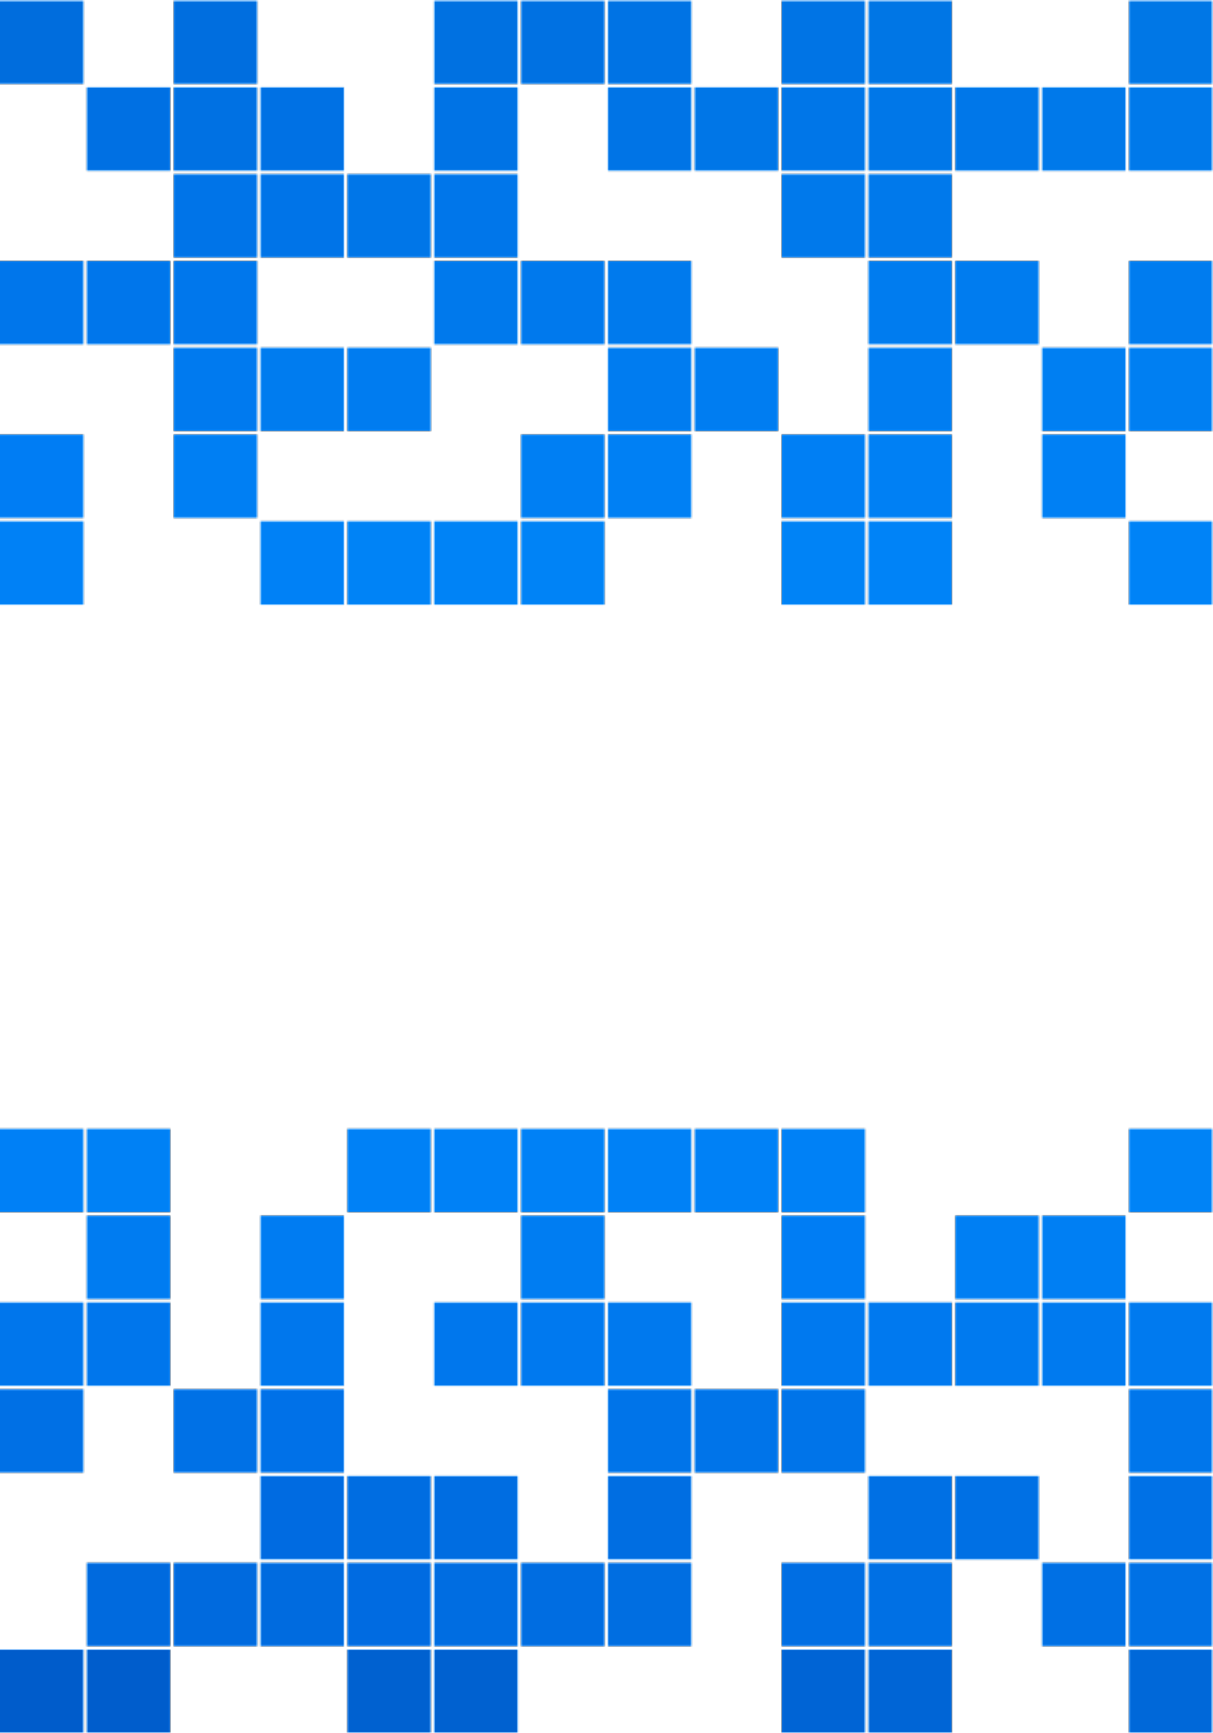
\includegraphics[width=\paperwidth]{background}};
\draw (current page.center) node [fill=steelblue!30!white,fill opacity=0.6,text opacity=1,inner sep=1cm]{\Huge\centering\bfseries\sffamily\parbox[c][][t]{\paperwidth}{\centering Naines blanches, étoiles à neutrons et étoiles étranges\\[15pt] % Book title
{\Large Les états exotiques de la matière dans les corps hyperdenses}\\[20pt] % Subtitle
{\huge Nicolas BELLEMONT et Théo TURLIN}}}; % Author name
\end{tikzpicture}
\vfill
\endgroup

%----------------------------------------------------------------------------------------
%	COPYRIGHT PAGE
%----------------------------------------------------------------------------------------

\newpage
~\vfill
\thispagestyle{empty}

\noindent Copyright \copyright\ 2013 John Smith\\ % Copyright notice

\noindent \textsc{Published by Publisher}\\ % Publisher

\noindent \textsc{book-website.com}\\ % URL

\noindent Licensed under the Creative Commons Attribution-NonCommercial 3.0 Unported License (the ``License''). You may not use this file except in compliance with the License. You may obtain a copy of the License at \url{http://creativecommons.org/licenses/by-nc/3.0}. Unless required by applicable law or agreed to in writing, software distributed under the License is distributed on an \textsc{``as is'' basis, without warranties or conditions of any kind}, either express or implied. See the License for the specific language governing permissions and limitations under the License.\\ % License information

\noindent \textit{First printing, March 2013} % Printing/edition date

%----------------------------------------------------------------------------------------
%	TABLE OF CONTENTS
%----------------------------------------------------------------------------------------

\usechapterimagefalse% If you don't want to include a chapter image, use this to toggle images off - it can be enabled later with \usechapterimagetrue

% \chapterimage{chapter_head.pdf} % Table of contents heading image

\pagestyle{empty} % No headers

\tableofcontents % Print the table of contents itself

\cleardoublepage% Forces the first chapter to start on an odd page so it's on the right

\pagestyle{fancy} % Print headers again

% %----------------------------------------------------------------------------------------
% %	PART
% %----------------------------------------------------------------------------------------

% \part{Part One}

%----------------------------------------------------------------------------------------
%	CHAPTER 1
%----------------------------------------------------------------------------------------

% \chapterimage{chapter_head.pdf} % Chapter heading image

\chapter{Quelques notions d'astronomie \ldots}

\section{Le cycle de la matière}
On appel \textit{Cycle de la matière galactique} les différentes étapes et états par lesquels transite la matière telle que nous la connaissons. C'est par ce cycle que notre univers s’enrichit en éléments lourd et que les étoiles ainsi que tous les objets visible sont créé, il va être question dans cette première partie de décrire ces différentes étapes et de mieux comprendre comment évolue la matière au sein de notre univers.
\n
Nous allons prendre comme point de départ de notre cycle le \textbf{milieu interstellaire}, il à une masse d'environ $5.10^{9}M_{\odot}$ et est constitué aux trois quart d'hydrogène, d'hélium à niveau d'un quart et que poussière pour ce qui est des dixième de pourcent restant (il constitue le réservoir de matière de notre univers). On considère que dans ce milieu la densité est environ d'une particule par $cm^3$, bien que cela soit extrêmement faible, certaines régions sont plus densément peuplée que d'autres a cela on rajoute l'hydrodynamique, l'auto gravité... on observe sur des périodes de temps assez faibles (quelques millions d'année) l'apparition de nuage moléculaire.\\ Ces nuages forment le milieu interstellaire \textbf{dense}, sa masse reste de l'ordre de $10^{9}M_{odot}$ mais sa composition à évolué pour être constitué à environ $75\%$ de dihydrogène (d’où le nom de nuage moléculaire). C'est à partir de ce moment que les choses vont s'emballer, les zones les plus denses des nuages vont attirer plus de matière à eux entraînant une augmentation de la densité etc... jusqu’à ce que l'instabilité gravitationnelle soit trop forte et que le nuage s’effondre sur lui même.\\
Il résulte de cet effondrement, la formation d'une \textbf{Proto-étoile}. Durant cette phase qui va durer quelques centaines de milliers d'années, la matière va continuer à tourner s'agglomérer autour du centre de gravité. Au fur et à mesurer de ce processus la proto-étoile va voir sa température augmenter, les particules du gaz vont s'échauffer continuellement jusqu’à atteindre une température critique qui permettra "l'allumage" de la réaction de fusion de l'hydrogène (plusieurs million de Kelvins), une \textbf{Étoile} est née.\\
Le cycle de vie d'une étoile est assez complexe, pour simplifier nous dirons que l'étoile fusionne de l’hydrogène en son sein et que cette réaction et à l'origine de la pression interne de l'étoile, pression qui vient compenser la force de gravité qui tend à faire s’effondrer l'étoile sur elle-même. Une fois que l'étoile à épuiser tout son hydrogène, la gravité va reprendre le dessus faire s’effondrer l'étoile, augmenter la pression et la température, réunissant les conditionsg pour fusionner l'hélium, stoppant effondrement etc...\footnote{Ce processus s’arrête au fer car aucune étoile ne peut fusionner le fer, en effet la fusion post fer consomme de l'énergie la ou la fusion pré fer en produisait.}.\\
Le cycle de vie d'une étoile est représenté par un diagramme HR (\textit{Hertzsprung-Russel}) qui permet de voir l'évolution d'une étoile le long de la séquence principale (où elle passera le plus clair de son existence) mais également de savoir quel objet astronomique il résultera de sa mort.\\
Une fois que l'étoile aura épuisé tout son carburant elle "mourra" sois en passant par la \textbf{Nébuleuse planétaire} sois en \textbf{Supernovæ} si l'étoile était suffisamment massive.\\
Ces deux phénomènes permettent de rendre au milieu interstellaire un grand nombre de nouvelle particules, enrichissant de manière considérable celui-ci et permettant l'apparition future d'objet céleste plus complexe en terme de composition.
\n
Nous rentrerons plus en détails sur les phénomènes de Nébuleuse planétaire et de Supernovæ dans les parties consacrées aux \textbf{Étoiles à neutron} et au \textbf{Naines blanches}, car nous verrons que dans la plupart des cas \footnote{La réalité astrophysique est bien plus complexe que cela et la manière de former certains objet de notre univers peut être assez exotique.} Ces objets sont le résultats des Nébuleuses et des Supernovæ.

\section{Les naines blanches}
\subsection{Nébuleuse planétaire}

Comme dit précédemment nous allons revenir sur le phénomène de Nébuleuse planétaire qui donne naissance à la plupart des naines blanches de l'Univers.\n
Pour commencer il faut savoir qu'une manière de classer les étoiles consiste à les ordonnée selon leurs masse, et donc on estime que seuls les étoiles de masse moyenne (C.à.D de moins de $10M_{\odot}$) donnent naissance à des Naines blanches. Le processus qui mène à la création d'une telle étoile est le suivant.\n
Tout d'abord comme nous l'avons vu dans notre introduction, une étoile va fusionner son hydrogène en hélium \footnote{On a généralement deux moyen d'y parvenir, sois par cycle proton-proton qui va par le biais du deutérium et du tritium/hélium 3 va donner de l'hélium 4, sois par le cycle CN0}\\
A partir de ce moment, la gravitation redevient alors la force dominante et l'étoile s’effondre sur elle même, les nouvelles conditions de pression et de température permette la fusion de l’hélium \footnote{Par un procédé appelé réaction triple alpha lorsque que la température aura atteint les $10^8 K$} cette fusion produit principalement du carbone et de l'oxygène et dégage une une importante quantité d'énergie qui ne se contente plus de contrebalancer l'effondrement gravitationnel mais qui fais gonfler l'étoile de manière impressionnante \footnote{On considère que lorsque le soleil entrera dans sa phase de géante rouge, sa taille aura tellement augmenter qu'il atteindra l'orbite de la Terre.} la transformant ainsi en géante rouge.\\
Les réserves d'hélium s’épuisant relativement vite, l’effondrement de l'étoile reprend assez vite, malheureusement pour la plupart des étoiles cet effondrement n'engendre pas une pression et une température suffisante pour amorcer le processus de fusion du carbone laissant l'étoile se réduire à un noyau solide de carbone et d'oxygène. Les couches externe de l'étoiles vont alors "rebondir" sur ce noyau. En réalité, le phénomène est plus complexe que ça et c'est par la pression de radiation que ces couches vont se faire souffler lors de la violente contraction du cœur de l'étoile.\\
Ce nuage de particule va donc lentement (à l'échelle de l'univers, en réalité ce nuage se déplace 100 000 $km/h$) se faire expulser allant ainsi alimenter le milieu interstellaire en élément plus riche, c'est la nébuleuse planétaire. Il ne reste plus alors que le noyau au centre de cet immense nuage et c'est ce "noyau" qui constitue la naine blanche.


\subsection{Quelques caractéristiques des naines blanches}
Une des première naine blanche à avoir été observé est Sirius B compagnon de l'étoile Sirius de la constellation du grand chien, ont avait remarqué en 1844 des anomalie dans la manière dont se déplaçait Sirius imaginé que ces anomalie pouvait être du à un compagnon encore invisible jusque la. Quelque année plus tard en 1862 ont réussi à observé Sirius B et a se rendre compte que cette étoile est bien une naine blanche.
\n

Bien que leurs tailles et leurs masse sois relativement variée, pour ce cours nous ferons l'approximation (partagée par la communauté scientifique) qu'une naine blanche
est un objet de la masse du soleil contenu dans un volume semblable à la Terre,
$$R\simeq 5000km\qquad M\simeq 10^{30}kg\qquad \rho\simeq 5.10^{6}g/cm^3$$
on note qu'elle figure parmi les objet les plus denses de l'univers.
La température au sein de ces monstres est de l'ordre de $10^7 K$ et le cœur de la naine, comme nous l'avons dit un peu plus haut, n'est plus constitué que des reste des réactions nucléaire, c'est à dire principalement de l'oxygène et du carbone, plus précisément d'un plasma constitué de noyau d'oxygène et d'électron.

\section{Les étoiles à neutrons}
\subsection{Supernovae\label{supernova}}
\begin{minipage}{0.3\textwidth}
    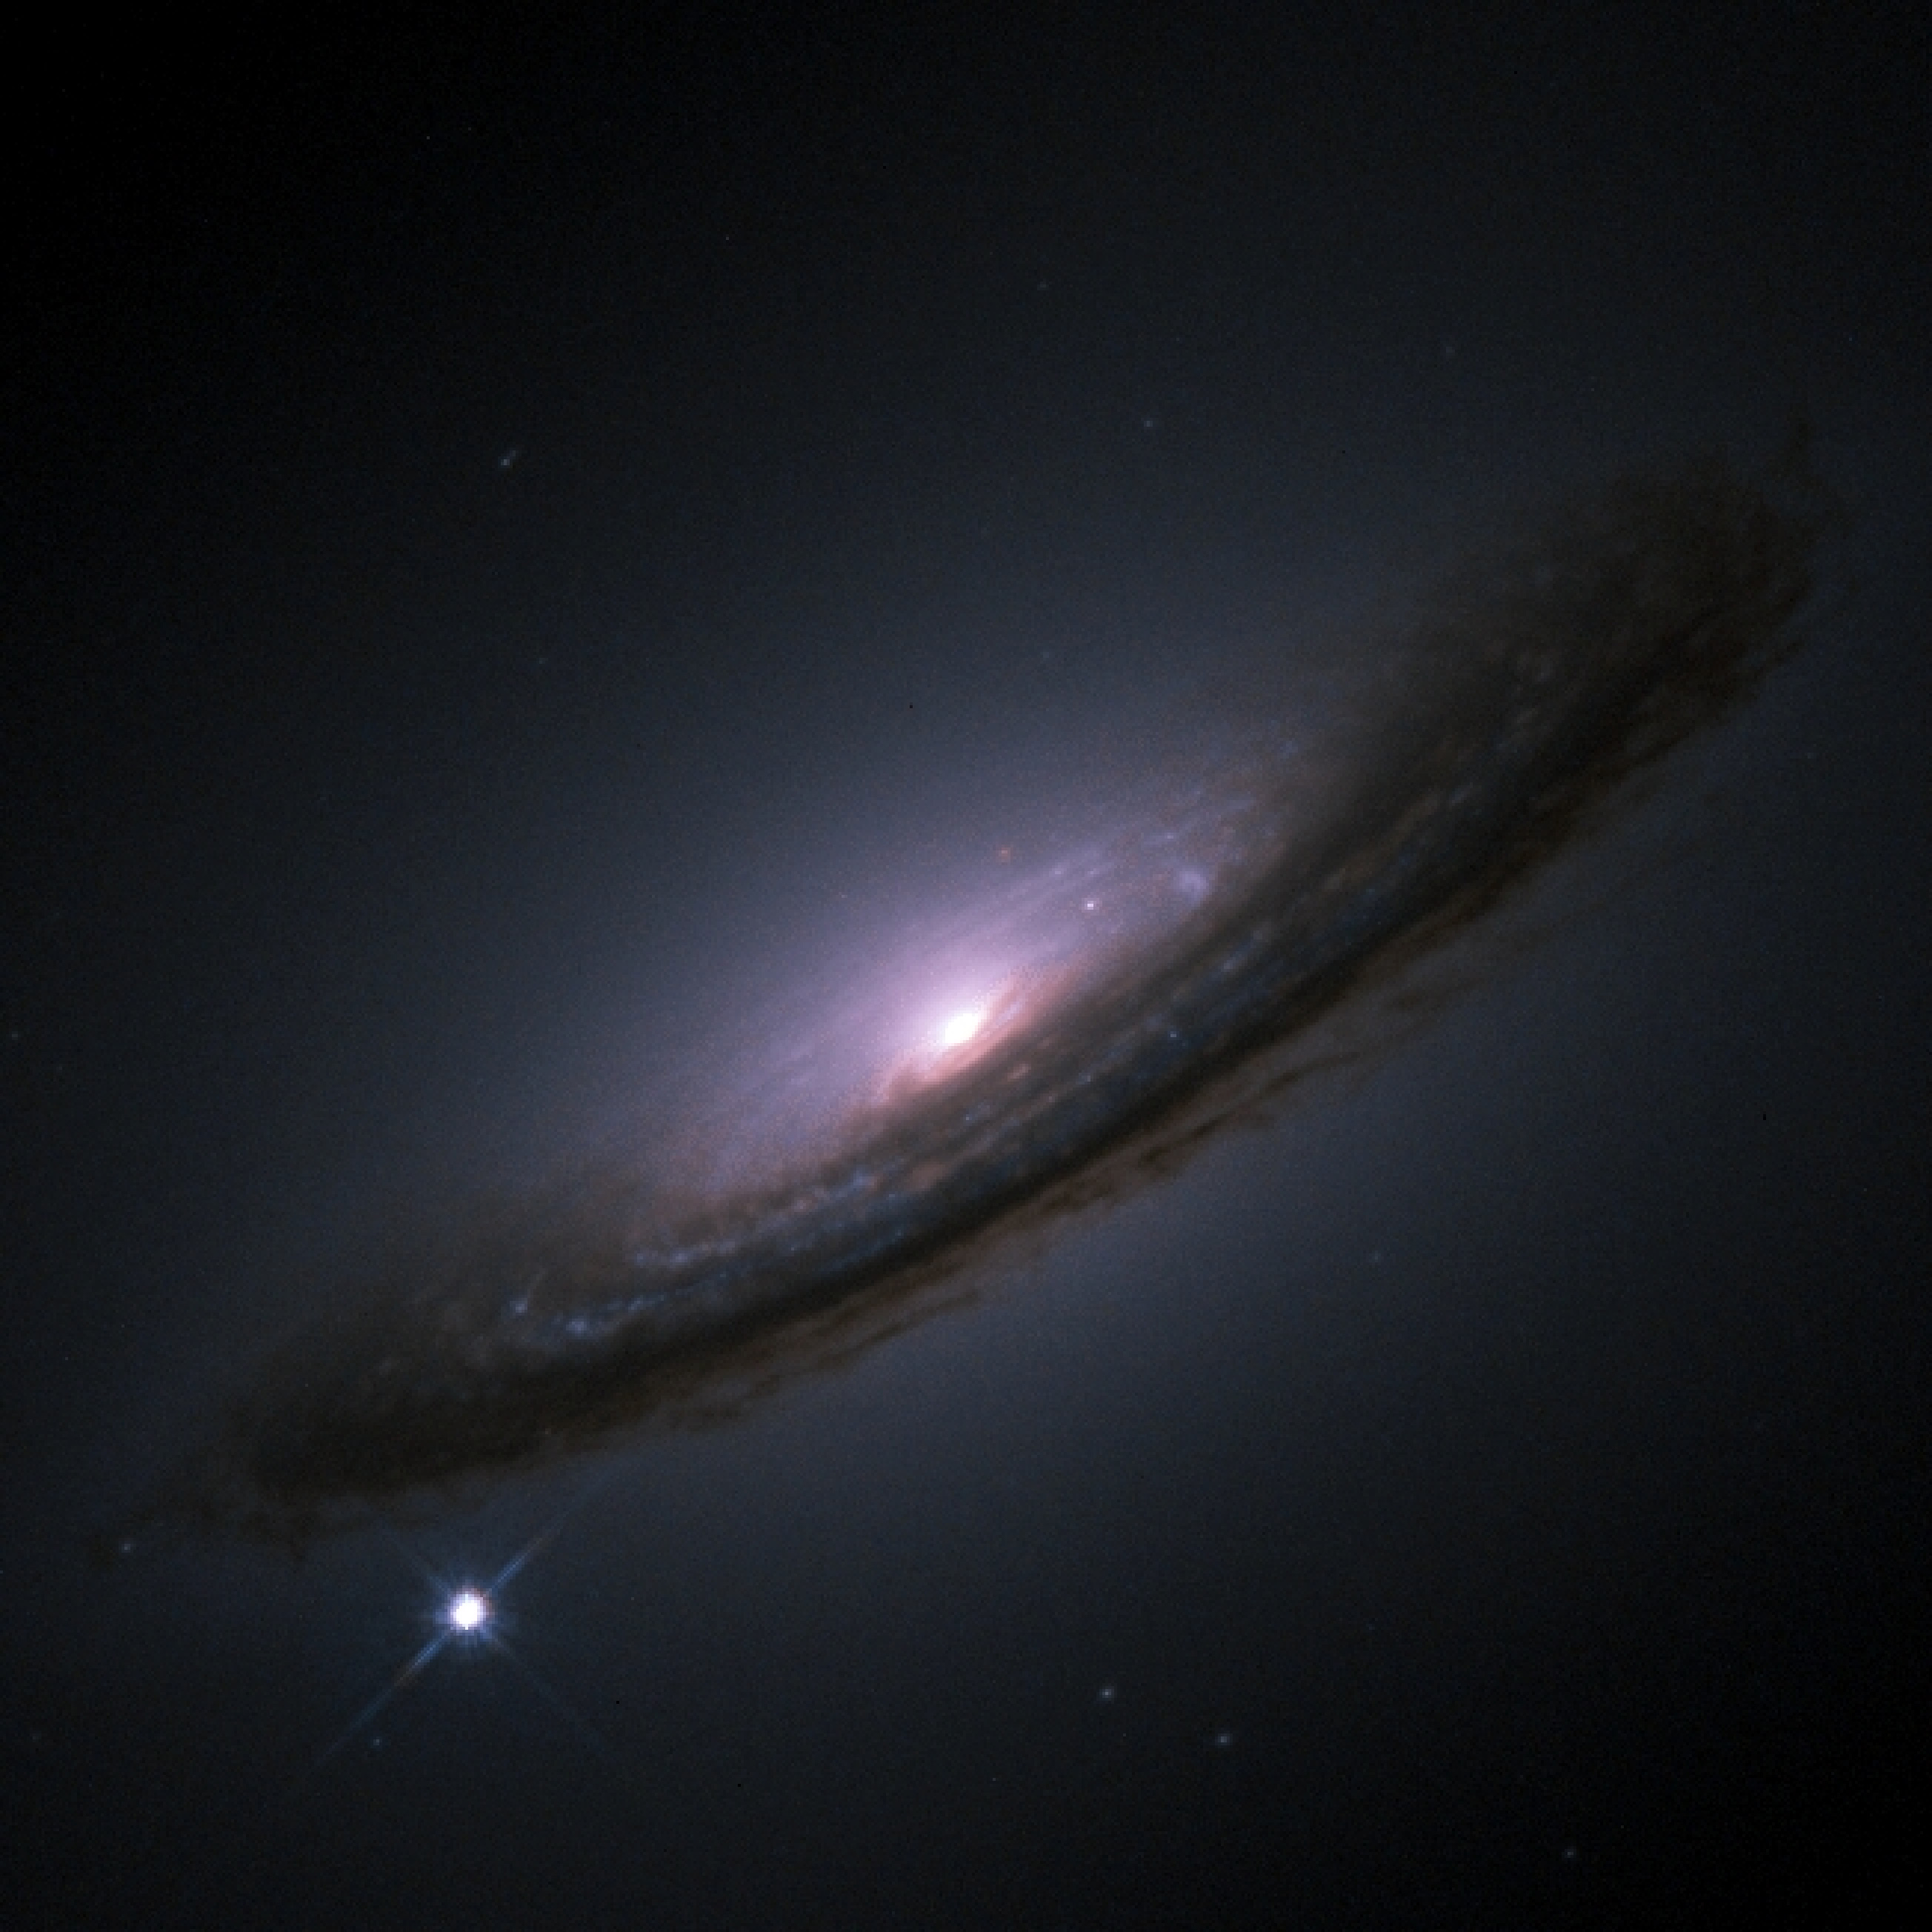
\includegraphics[width=1\textwidth]{Pictures/SN1994D.jpg}
    \captionof{figure}{SN 1994D est une supernova de type Ia en train de briller en dehors de sa galaxie mère, NCG 4526.\\Credits : NASA}
\end{minipage}
\hspace{0.025\textwidth}
\begin{minipage}{0.35\textwidth}
    Il existe deux principaux phénomènes menant à une supernova, que sont l'explosion thermonucléaire d'une naine blanche, appelée supernova de type Ia, et l'effondrement du c{\oe}ur, appelée supernova de type Ib, Ic ou II suivant la composition de l'étoile. \cite{sup}
\end{minipage}
\hspace{0.025\textwidth}
\begin{minipage}{0.3\textwidth}
    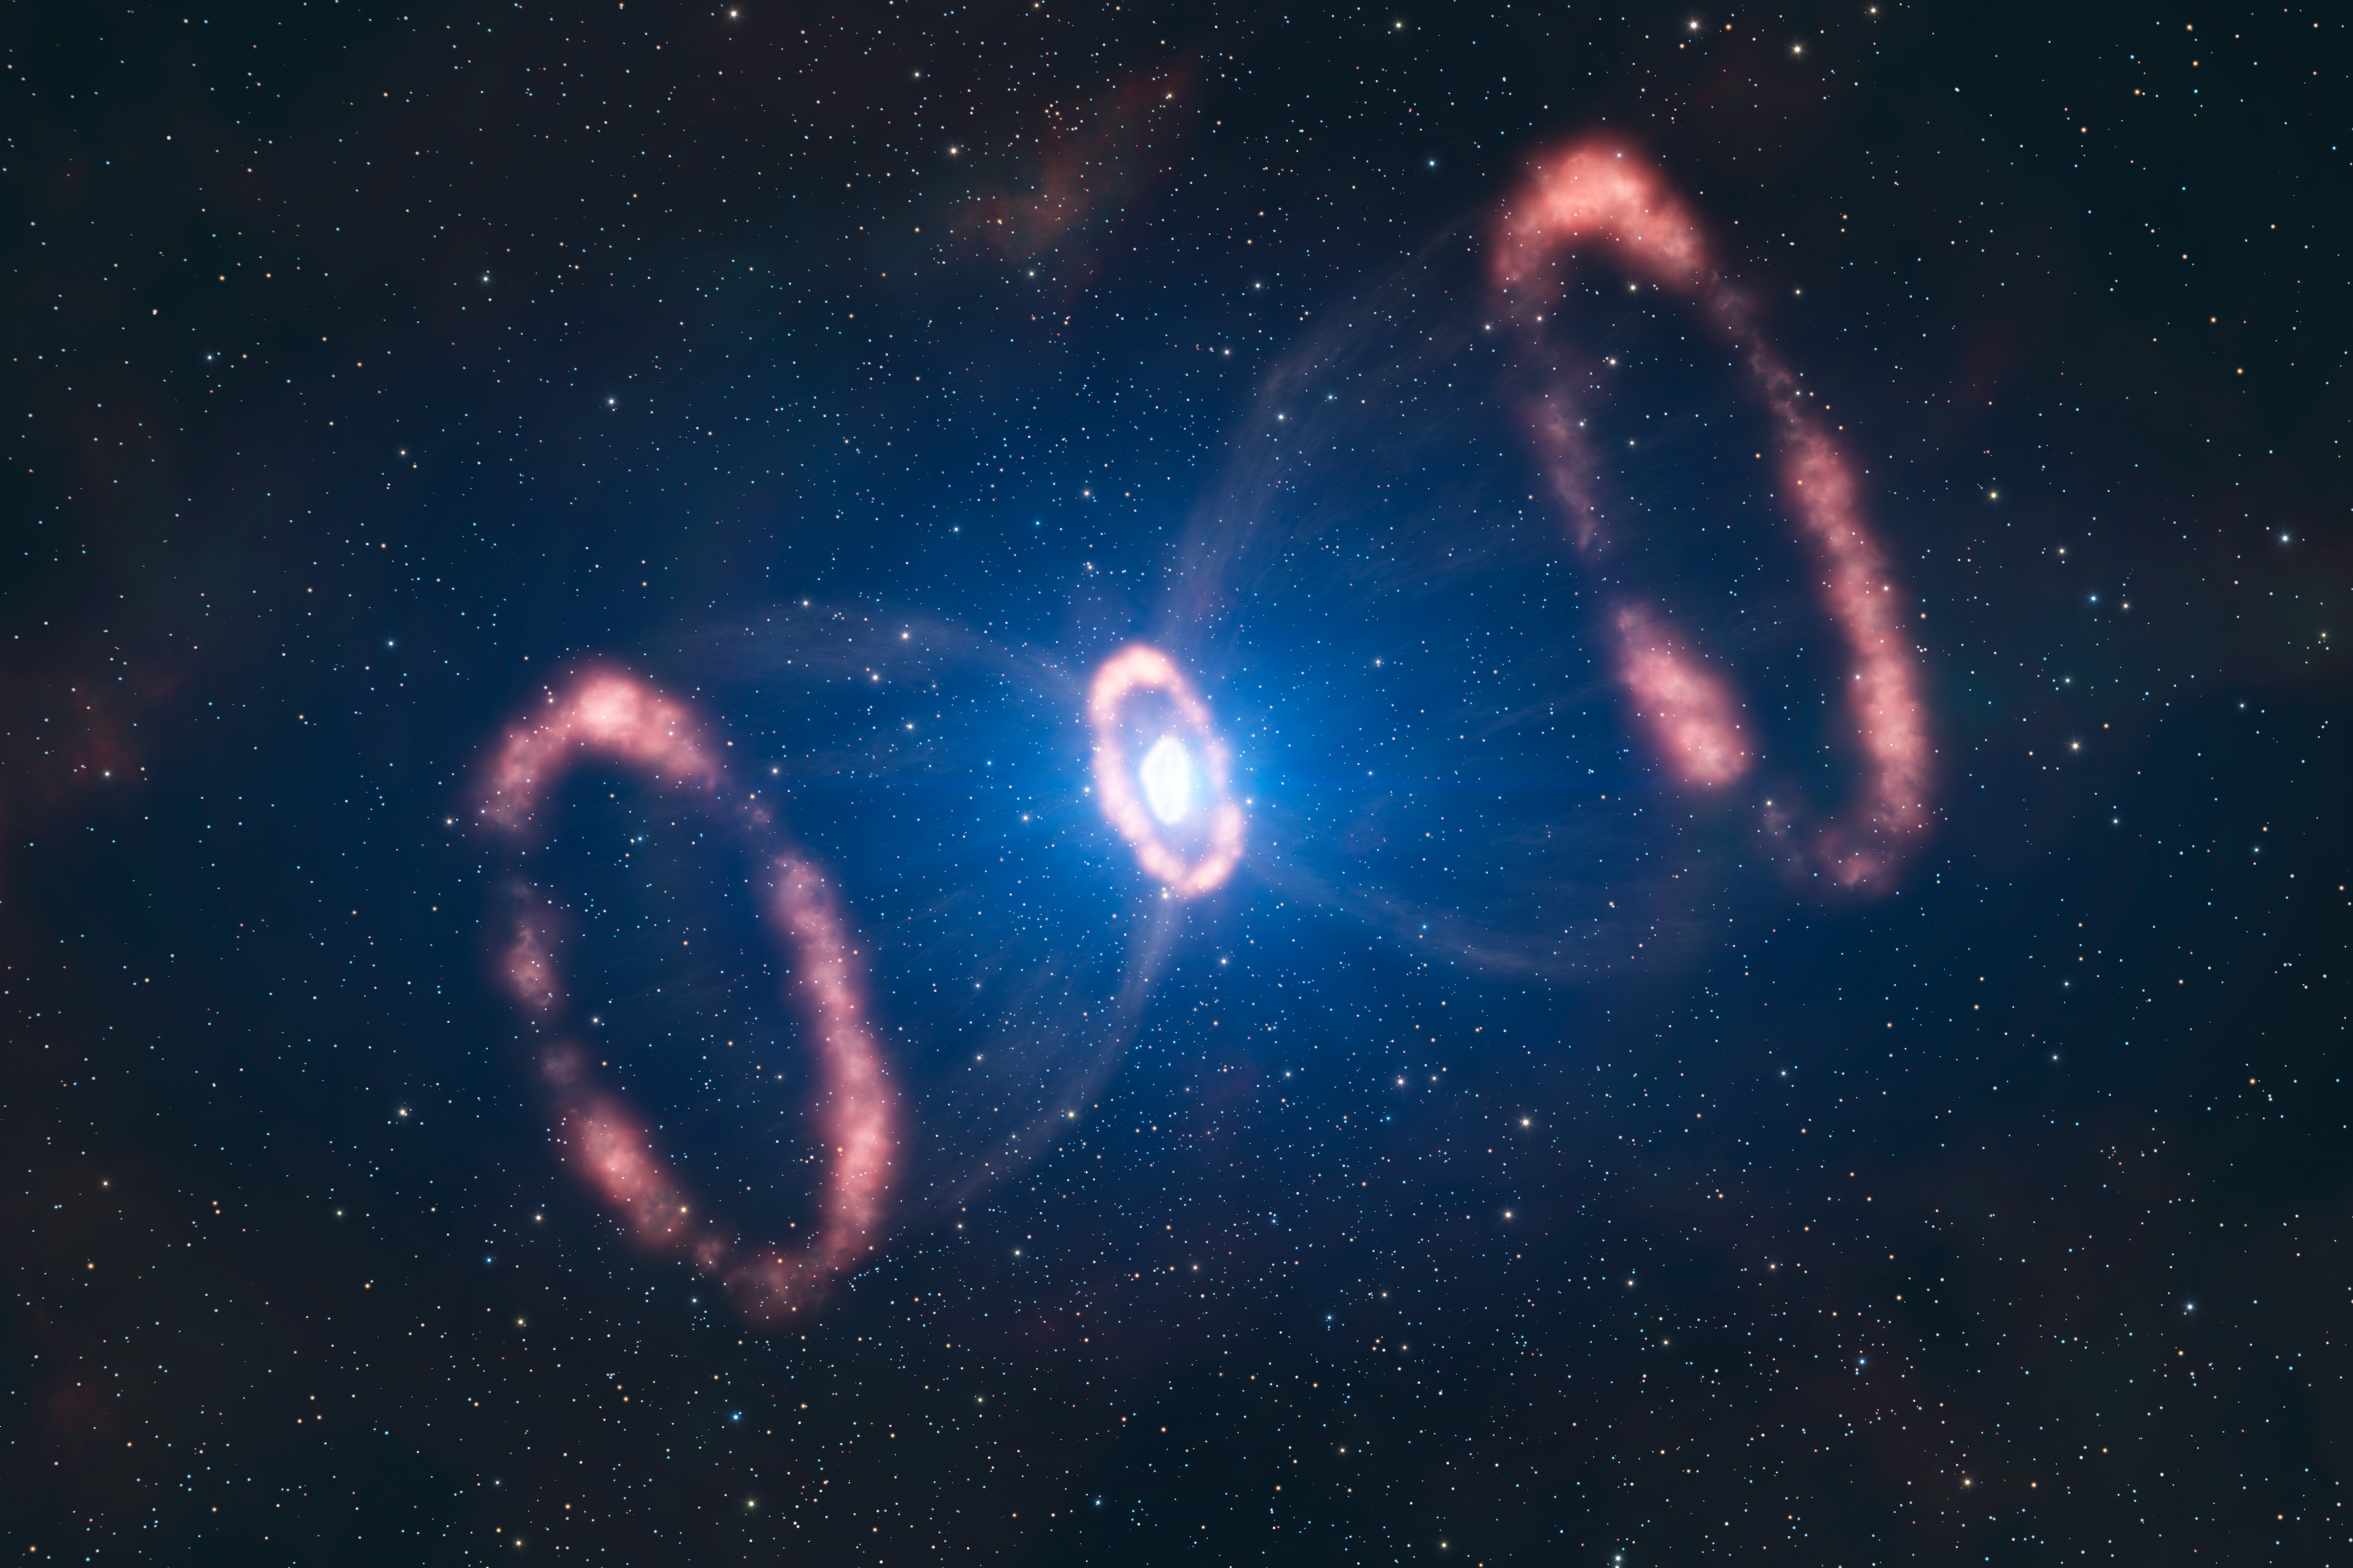
\includegraphics[width=1\textwidth]{Pictures/SN1987A.jpg}
    \captionof{figure}{Représentation d'artiste de SN 1987A.\\Crédits : ESO}
\end{minipage}

\subsubsection{Supernova par explosion thermonucléaire \cite{supth}\cite{sup1a}}
Ce type de réaction ne peut s'initier que dans un système binaire, composé d'une naine blanche et d'une autre étoile, suffisament compact pour que l'étoile puisse déverser du gaz sur la naine blanche. L'explosion est amorcée par effondrement gravitationnel de celle-ci. Les réactions nucléaires démarrent et ne prennent que quelques instants, créant des élements allant jusqu'au nickel. Sous la pression thermique crée par la naine blanche, les couches supérieures sont soufflées, ce qui lève la dégénérescence des couches de la naine blanche, qui sont à leur tours soufflées. Dans ce procédé, l'étoile est complètement désintégrée.

\subsubsection{Supernova à effondrement de coeur \cite{supec}\cite{sup2}}
Ce type de supernova concerne les étoiles dont la masse est comprise entre \(10M_\odot\) et \(40M_\odot\), au-delà de cette masse critique, une étoile est supposé s'effondrée directement en un trou noir. Pour pouvoir exploser en supernova, une étoile massive doit fusionner tout ses élements jusqu'au fer, qui est un élément inerte.
\begin{remark}
    Un élément inerte est un élément dont on ne peut extraire de l'énergie ni par fusion, ni par fusion 
\end{remark}

Une fois le coeur de fer crée, le cycle de la supernova s'enclenche. Tout d'abord, le coeur de fer s'effondre sur lui-même, entrainant de par le fait une augmentation de sa température et de sa densité, ce qui favorise les captures électroniques. Les électrons vont réagir avec les protons des atomes de fer et former des neutrons et des neutrinos. la diminution du nombre d'électrons entraine une diminution de la pression de dégénérescence des électrons dans le coeur de l'étoile.\n

\begin{definition}[Pression de dégénérescence]
    On appelle pression de dégénérescence la pression à partir de laquelle la matière se comporte comme un gaz et où la force nucléaire forte empêche sa densité d'augmenter.
\end{definition}

À ce moment, la gravition du c{\oe}ur l'emporte sur la pression de dégénérescence, et il s'effondre sur lui-même, quasiment en chute libre jusqu'à ce que les captures électroniques se terminent, que toute la matière soit transformée en neutrons et que la densité soit de l'ordre de \(10^{17}kg.m^{-3}\). Le c{\oe}ur continue de s'effondrer jusqu'à atteindre la densité atomique, soit environ \(2\cdot 10^5kg.m^{-3}\). Cet effondrement ce fait à une vitesse moyenne de \(70\ 000km.s^{-1}\simeq 0.23c\). À ce moment, le c{\oe}ur ne mesure que quelques kilomètres de diamètre.\n
La vitesse de l'effondrement est telle que les couches externes de l'étoile n'ont pas le temps de ``suivre'' le c{\oe}ur, ce qui crée une zone de vide entre celles-ci et le noyau. Les couches externes s'effondrent alors sur le noyau, mais celui-ci ne peut être plus compact. Lorsqu'elles touchent le noyau de neutrons, elles rebondissent alors sur ce dernier, ce qui crée le choc.\n
Le choc se propage a environ \(0.25c\) sur une centaine de kilomètres avant de s'arreter, son énergie etant consommée par les captures électroniques et la dissociation des atomes de fer, mais les neutrinos émis par les réactions thermonucléaires permettent de faire repartir ce dernier. Il se propage à travers les différentes couches de l'étoile, sa vitesse augmentant à chaque interface, pour atteindre environ \(0.5c\) à la surface. Cela éjecte la matière et l'étoile devient alors une supernova.\n
La luminosité de cette explosion peut atteindre 100 milliards de fois la luminosité solaire, mais cette luminosité ne correspond qu'a \(0.01\%\) de l'énergie de la supernova, \(99\%\) de celle-ci étant emportée par les neutrinos, ce qui reste est converti en énergie cinétique pour l'objet résultant de cette supernova.\n
Les objets compacts résultants de cette dernière varie en fonction de la masse de l'étoile de départ. Si cette dernière était comprise entre \(8M_\odot\) et \(15M_\odot\), alors le coeur devient une étoile à neutrons, au-delà de cette masse de \(15M_\odot\), la masse initiale de l'étoile n'est pas suffisante pour déterminer si le résultat sera une étoile à neutrons ou un trou noir.

\subsection{Caractéristique d'une étoile à neutrons}\label{neutron}
Ce type d'étoiles à une masse allant de \(1.4M_\odot\) à \(2.16M_\odot\) pour un rayon d'une dizaine de kilomètres, elle possède donc une densité de l'ordre de \(3\cdot 10^{26}\ kg.m^{-3}\).
\begin{remark}
    Une boite d'allumette en ``étoile à neutron'' pèse 3 milliards de tonnes
\end{remark}
Une fois formée, elle ne produit plus de chaleur. Sa temperature lors de sa formation atteint les \(10^{11}K\) mais elle décroit rapidement pour atteindre \(5.10^6K\)

\chapter{Les états exotiques de la matière}

La matière dégénérée est un état particulier de la matière fermionique. Cette état extrêmement dense est composé de particules qui peuplent les états de haute énergie cinétique, afin de satisfaire le principe d'exclusion de Pauli. En effet, ce dernier interdit à deux fermions de se trouver dans le même état quantique. Or lorsque la densité de matière augmente, certaines fonctions d'ondes finissent par se superposer entre différents fermions. La pression de dégénérescence s'applique dès lors que les fonctions d'ondes qui tentent de se superposer concernent deux fermions dans le même état. Cet état de la matière est décrite par un gaz de Fermi.

\section{Théorie des naines blanches}
Nous avons vus que les étoiles de la séquence principales sont en équilibre car les réactions nucléaires qui se produisent dans leurs cœurs permettent de contrebalancer l'effondrement gravitationnel, cependant qu'en est-il des naines blanches? pendant longtemps les scientifiques se sont posé la question étant donnée que nous savons les naines blanches exemptent de toutes réactions nucléaires en plus d'avoir à subir d'incroyable force de pression gravitationnelle.\\
Un élément de réponse à été apporter en 1925 par le britannique Ralph Fowler, qui propose d'appliquer les principes de la mécaniques quantiques au gaz d'électrons présent dans le noyau des naines blanches. Ce que propose Fowler c'est que les électron représente en réalité un gaz quantique dégénéré et que ce gaz induit une pression quantique qui vient assurer la stabilité de la naine blanche.\\
Le but de la partie d'aujourd'hui va être de retrouver ces résultats et de redémontrer qu'effectivement la stabilité d'une naine blanche provient d'une pression quantique induites par un gaz d'électrons dégénéré relativistes.
\subsection{Gaz dégénéré...}

\begin{itemize}
  \item Pour commencer l'énergie potentielle gravitationnelle d'un corps de masse M et de dimension R vaut $E_g = -G \frac{M^2}{R}$
  \item Pour se faire une idée de l’intensité de ces force on imagine un accroissement DR de l'objet $dE_g = G \frac{M^2}{R^2}dR$
  \item l'augmentation d'énergie correspond à un travail $\delta W = -dE_g$ avec $dW  =P_gdV = P_g 4\pi R^2 dR$
  \item on obtient au final $P_g\simeq -\frac{G}{4_pi}\frac{M^2}{R^4} = -\frac{6.67.10^{-11}}{4\pi}\frac{M^2}{R^4} = \boxed{-10^{33} Pa}$
\end{itemize}
\n
\begin{itemize}
  \item Naine blanche rayonne $\rightarrow$ perte d'énergie et donc refroidissement
  \item Refroidissement entraîne théoriquement une recombinaisons noyaux/électrons
  \item Calcul du nombre de noyaux par unité de volume
\end{itemize}

$$\frac{N}{V}\simeq \frac{\rho}{A}*N_A \simeq 2.10^{29}cm^{-3}$$
\begin{itemize}
  \item En inversant on à le volume dispose disponible pour chaque noyaux $5.10^{-6}A$
  \item Volume occupé par un atome? 1 million de fois plus grand
  \item Aucun phénomène physique connu capable de contrebalancer les forces gravitationnelle pour augmenter à ce point le volume.
\end{itemize}
\n
On s’intéresse à la température de Fermi (température de dégénérescence) du gaz d'électrons
\begin{itemize}
  \item Même manière de calculer que pendant le cours de physique des matériaux
  $$T_F = \frac{\hbar^2}{2m_e K}\left(3\pi^2 \frac{N_e}{V}\right)^{\frac{2}{3}}$$
  \item Température de Fermi $\boxed{5.10^9 K}$
  \item Avec $\frac{N_e}{V}\simeq \frac{\rho}{A}*Z*N_A = 1.5.10^{30}cm^{-3}$
  \item Température du gaz d'électron bien en deçà de la température de Fermi $\rightarrow$ Gaz d'électron totalement dégénérée.
\end{itemize}
\n

\begin{itemize}
  \item Pression d'un gaz de fermions dégénérée $$\frac{2}{15\pi^2\hbar^3}(2m_e)^{\frac{3}{2}}(kT_f)^{\frac{5}{2}}$$
  $\hbar = 1.054.10^{-34}$
  $9.1.10^{-31}$
  \item Pression du gaz d'électrons $\simeq \boxed{10^{22} Pa}$
  \item On voit qu'un gaz d'électron dégénérée ne suffit pas à expliquer la stabilité de la naine blanche, la pression n'est pas assez forte.
\end{itemize}

\subsection{... d'électrons relativistes}
\begin{itemize}
  \item Toujours par rapport au cours de matériaux on à les énergie mises en jeu qui valent $E = k*T_F \simeq \boxed{10^5 eV}$
  \item Les électrons sont relativistes : $E = \sqrt{p^2c^2 + m^2c^4}$
  \item On en profite pour calculer l'impulsion de Fermi $ \sqrt{\frac{E^2 - m^2c^4}{c^2}} = 3.3.10^{-4}$
  \item travailler avec des formules relativistes de gaz dégénérée afin de trouver la condition d'équilibre de la naine blanche.
\end{itemize}
\n
\begin{itemize}
  \item On peut montrer que la pression d'un gaz relativiste est donnée par $P = \frac{J}{V}$ avec J le grand potentiel (potentiel de la distribution micro canonique).
  \item Les formules sont assez complexe et assommantes, mais pour des gaz ou le gaz est complètement dégénérée (température très faible devant la température de Fermi), le grand potentiel s'écrit :
  $$J = - \frac{V}{3\pi^2\hbar^3}\int_0^{p_F} p^3 \frac{dE}{dp} dp$$
  \item La pression des particules relativiste s'écrit donc $$P = \frac{c^2}{3\pi^2\hbar^3}\int_0^{p_F} \frac{p^4}{\sqrt{p^2c^2 + m^2c^4}} dp $$
  \item on pose le chgt de variable $x = \frac{p}{mc}$
  \begin{eqnarray*}
    P &=& \frac{c^2}{3\pi^2\hbar^3}\int_0^{x_F} \frac{x^4 m^4 c^4}{\sqrt{x^2 m^2 c^4 + m^2c^4}}mcdx\\
    &=&\frac{c^2}{3\pi^2\hbar^3}\int_0^{x_F}\frac{x^4m^5c^5}{\sqrt{m^2c^4(x^2 + 1)}}dx\\
    &=&\frac{m^4c^5}{3\pi^2\hbar^3}\int_0^{x_F} \frac{x^4}{\sqrt{x^2 + 1}}\\
    &=& \boxed{\frac{c}{12\pi^2 \hbar^3}p_F^4\left[1 - \frac{m^2 c^2}{p_F^2}\right]}
  \end{eqnarray*}
  \item On calcule et on obtient une pression pour le gaz dégénérée d'électron relativiste de $\boxed{10^{36}Pa}$

\end{itemize}
Au arrondi près et au erreurs de calculs, on trouve une pression bien supérieur à celle du seuls gaz d’électrons dégénérée et ont voit bien que cette pression est suffisante pour permettre de contrebalancer la pression gravitationnelle et maintenir la naine blanche en équilibre.


\section{Étoiles à neutrons}
\subsection{Détermination de la pression gravitationnelle et de la pression de dégénérescence}
La stabilité d'une étoile résulte de l'équilibre entre les forces gravitationnelles qui tendent à compresser l'étoile et la pression du gaz constituant cette dernière qui tend à s'étendre dans tout l'espace disponible du fait de sa pression. L'effondrement de l'étoile sur elle-même s'arrente quand les processus physiques internes (transformation d'un couple proton-électron en un neutron) créent une pression suffisante pour compenser les forces gravitationnelles. Afin de comparer les deux phénomènes, nous allons calculer une ``pression gravitationnelle''. Cette pression gravitationnelle s'obtient de la manière suivante : 
\begin{eqnarray*}
    P_G&=&\frac{F}{S}\\
    &=&\frac{-\frac{GM^2}{R^2}}{4\pi R^2}\\
    &=&-\frac{G}{4\pi}\frac{M^2}{R^4}
\end{eqnarray*}
Une chose importante à constater est que cette pression est négative, cela traduit le fait que la pression gravitationnelle tend à compresser le système.\n
Nous allons désormais calculer la température de Fermi du gaz de neutron. Pour cela nous allons avoir besoin du rapport \(\frac{N}{V}\)
\[\frac{N}{V}=\frac{\frac{M}{m_n}}{\frac{4}{3}\pi R^3}=\frac{3M}{4m_n\pi R^3}\]
Nous pouvons donc maintenant calculer la température de Fermi de l'étoile
\begin{eqnarray*}
    T_F&=&\frac{E_F}{k_B}\\
    &=&\frac{\hbar^2}{2k_Bm_n}\left(3\pi^2\frac{N}{V}\right)^{\frac{3}{2}}\\
    &\simeq&10^{10}K
\end{eqnarray*}
On constate que celle-ci est légèrement inférieure à celle de l'étoile lors de sa formation, mais qu'elle devient rapidement beaucoup plus grande que cette dernière, puisque l'étoile refroidit très vite\ref{neutron}. Une fois l'étoile stabilisée, le rapport \(\frac{T}{T_F}\) est très inférieur à 1, donc le gaz de neutron est totalement dégénéré. Or la pression d'un gaz de fermions dégénéré tend vers une limite non-nulle lorsque \(T\) devient très inférieure à \(T_F\). 
\n
La formule pour la pression de dégénérescence d'un gaz de neutron est \[P_0=\frac{2\hbar^2}{m_n}\left(\frac{\rho}{m_n}\right)^{\frac{5}{3}}\]

\subsection{Condition d'équilibre d'une étoile à neutron et relation rayon-masse}
Pour que l'étoile soit en équilibre les deux pressions doivent se compenser.

\begin{eqnarray*}
    P_0+P_G&=&0\\
    \frac{2\hbar^2}{m_n}\left(\frac{3M}{4\pi R^3}\right)^{\frac{5}{3}}&=&\frac{G}{4\pi}\frac{M^2}{R^4}\\
    \frac{2h^2}{4\pi^2m_n}\left(\frac{3M}{4\pi}\right)^{\frac{5}{3}}\frac{1}{R^5}&=&\frac{G}{4\pi}\frac{M^2}{R^4}\\
    \frac{2h^2}{\pi m_n}\left(\frac{3}{4\pi}\right)^{\frac{5}{3}}\frac{M^{\frac{5}{3}}}{GM^2}&=&R\\
    R&=&\frac{4\hbar^2}{Gm_n}\left(\frac{3}{4\pi}\right)^{\frac{5}{3}}\frac{1}{M^{\frac{1}{3}}}
\end{eqnarray*}

On peut réécrire cette condition sous la forme \(RM^{\frac{1}{3}}=cst\). Nous obtenons donc une relation simple entre le rayon d'une étoile à neutrons et sa masse.

%----------------------------------------------------------------------------------------
%	BIBLIOGRAPHY
%----------------------------------------------------------------------------------------

\chapter*{Bibliographie}
\addcontentsline{toc}{chapter}{\textcolor{steelblue}{Bibliographie}}
\section*{Sites web}
\addcontentsline{toc}{section}{Sites web}
\printbibliography[heading=bibempty,type=other]

%----------------------------------------------------------------------------------------
%	INDEX
%----------------------------------------------------------------------------------------

\cleardoublepage
\phantomsection
\setlength{\columnsep}{0.75cm}
\addcontentsline{toc}{chapter}{\textcolor{steelblue}{Index}}
\printindex

%----------------------------------------------------------------------------------------

\end{document}
